%%%%%%%%%%%%%%%%%%%%%%%%%%%%%%%%%%%%%%%%%%%%%%%%%%%%%%%%%%%%%%%%%%%%%%%%%%%%%%%%%%%%%%%%%%%%%%%%%%%
%%%%%%%%%%%%%%%%%%%%%%%%%%%%%%%%%%%%%%%%%%%%%%%%%%%%%%%%%%%%%%%%%%%%%%%%%%%%%%%%%%%%%%%%%%%%%%%%%%%
%%%%%%%%%%%%%%%%%%%%%%%%%%%%%%%%%%%%%%%%%%%%%%%%%%%%%%%%%%%%%%%%%%%%%%%%%%%%%%%%%%%%%%%%%%%%%%%%%%%
\documentclass[12pt,dvipdfmx]{beamer}
%%%%%%%%%%%%%%%%%%%%%%%%%%%%%%%%%%%%%%%%%%%%%%%%%%%%%%%%%%%%%%%%%%%%%%%%%%%%%%%%%%%%%%%%%%%%%%%%%%%%%%
% pdfの栞・プロパティの字化けを防ぐ
\usepackage{atbegshi}
%\AtBeginShipoutFirst{\special{pdf:tounicode 90ms-RKSJ-UCS2}} %Windows
\AtBeginShipoutFirst{\special{pdf:tounicode EUC-UCS2}} %Linux, Mac
\usepackage{hyperref}
%%%%%%%%%%%%%%%%%%%%%%%%%%%%%%%%%%%%%%%%%%%%%%%%%%%%%%%%%%%%%%%%%%%%%%%%%%%%%%%%%%%%%%%%%%%%%%%%%%%%%%
%%%
%%% テーマの指定、省略時は default になる
%%%

 % フレームの指定、省略可
%%%%%%%%%%%%%%%%%%%%%%%%%%%% THEME
  %\usetheme{AnnArbor}
  %\usetheme{Antibes}
  %\usetheme{Bergen}
  %\usetheme{Berkeley}
  %\usetheme{Berlin}
  \usetheme{Boadilla}
  %\usetheme{boxes}
  %\usetheme{CambridgeUS}
  %\usetheme{Copenhagen}
  %\usetheme{Darmstadt}
  %\usetheme{default}
  %\usetheme{Dresden}
  %\usetheme{Frankfurt}
  %\usetheme{Goettingen}
  %\usetheme{Hannover}
  %\usetheme{Ilmenau}
  %\usetheme{JuanLesPins}
  %\usetheme{Luebeck}
  %\usetheme{Madrid}
  %\usetheme{Malmoe}
  %\usetheme{Marburg}
  %\usetheme{Montpellier}
  %\usetheme{PaloAlto}
  %\usetheme{Pittsburgh}
  %\usetheme{Rochester}
  %\usetheme{Singapore}
  %\usetheme{Szeged}
  %\usetheme{Warsaw}

% 省略可
%%%%%%%%%%%%%%%%%%%%%%%%%%%% COLOR THEME
  %\usecolortheme{albatross}
  %\usecolortheme{beetle}
  %\usecolortheme{crane}
  %\usecolortheme{default}
  %\usecolortheme{dolphin}
  %\usecolortheme{dove}
  %\usecolortheme{fly}
  %\usecolortheme{lily}
  %\usecolortheme{orchid}
  %\usecolortheme{rose}
  %\usecolortheme{seagull}
  %\usecolortheme{seahorse}
  %\usecolortheme{sidebartab}
  %\usecolortheme{structure}
  %\usecolortheme{whale}

% ヘッダ、フッタ、フレーム等を指定、省略可
  %%%%%%%%%%%%%%%%%%%%%%%%%%%% OUTER THEME
  %\useoutertheme{default}
  %\useoutertheme{infolines}
  %\useoutertheme{miniframes}
  %\useoutertheme{shadow}
  %\useoutertheme{sidebar}
  %\useoutertheme{smoothbars}
  %\useoutertheme{smoothtree}
  %\useoutertheme{split}
  %\useoutertheme{tree}

% タイトル、section, itemize/enumerate 環境、
% theorem 環境、図, 参考文献などのスタイルを指定、
% 省略可
  %%%%%%%%%%%%%%%%%%%%%%%%%%%% INNER THEME
  %\useinnertheme{circles}
  %\useinnertheme{default}
  %\useinnertheme{inmargin}
  \useinnertheme{rectangles}
  %\useinnertheme{rounded}


%\usefonttheme{}	% 省略可
%\logo{}		% 省略可

%%%%%%%%%%%%%%%%%%%%%%%%%%%%%%%%%%%%%%%%%%%%%%%%%%%%%%%%%%%%%%%%%%%%%%%%%%%%%%%%%%%%%%%%%%%%%%%%%%%
%%%%%%%%%%%%%%%%%%%%%%%%%%%%%%%%%%%%%%%%%%%%%%%%%%%%%%%%%%%%%%%%%%%%%%%%%%%%%%%%%%%%%%%%%%%%%%%%%%%
%%%%%%%%%%%%%%%%%%%%%%%%%%%%%%%%%%%%%%%%%%%%%%%%%%%%%%%%%%%%%%%%%%%%%%%%%%%%%%%%%%%%%%%%%%%%%%%%%%%
% navi. symbolsは目立たないが,dvipdfmxを使うと機能しないので非表示に
\setbeamertemplate{navigation symbols}{}

% 各種パッケージ
\usepackage{graphicx}
%\usepackage{url,cite}
\usepackage{amsmath}
\usepackage{amsthm} \theoremstyle{definition} %theorem環境が斜体になるので注意
\usepackage{amssymb} % AMS-TeX
\usepackage{setspace}

% \AtBeginSection[] % Do nothing for \section*
% { \begin{frame}<beamer> \frametitle{}
%    \tableofcontents[currentsection,subsectionstyle=hide]
%  \end{frame} } 

%appendixをページカウントしない
\newcommand{\backupbegin}{
   \newcounter{framenumberappendix}
   \setcounter{framenumberappendix}{\value{framenumber}}
}
\newcommand{\backupend}{
   \addtocounter{framenumberappendix}{-\value{framenumber}}
   \addtocounter{framenumber}{\value{framenumberappendix}} 
}

%%%%%%%%%%%%%%%%%%%%%%%%%%%%%%%%%%%%%%%%%%%%%%%%%%%%%%%%%%%%%%%%%%%%%%%%%%%%%%%%%%%%%%%%%%%%%%%%%%%%%%
% 本文・数式フォント
%\usepackage{palatino,mathpazo}
%\usepackage{times,mathptmx}
\usepackage[varg]{txfonts}
%\usepackage[varg]{pxfonts}

% \mathcal(\cal)の扱い
%\DeclareMathAlphabet{\mathcal}{OMS}{cmsy}{m}{n} %computer modern
%\DeclareMathAlphabet{\mathcal}{OMS}{txsy}{m}{n} %txfont
%\usepackage[psamsfonts]{eucal} % euler

% mathptmx時に数式モードのvをtxfontから借りる
% \DeclareSymbolFont{lettersA}{U}{txmia}{m}{it}
% \SetSymbolFont{lettersA}{bold}{U}{txmia}{bx}{it}
% \DeclareFontSubstitution{U}{txmia}{m}{it}
% \DeclareMathSymbol{v}{\mathalpha}{lettersA}{"33} %"

\usepackage{multirow}

%上線 widebar, Widebar
\usepackage{accents}
\makeatletter
\def\widebar{\accentset{{\cc@style\underline{\mskip11mu}}}}
\makeatother


%%%%%%%%%%%%%%%%%%%%%%%%%%%%%%%%%%%%%%%%%%%%%%%%%%%%%%%%%%%%%%%%%%%%%%%%%%%%%%%%%%%%%%%%%%%%%%%%%%%%%%

% 定理環境
% \newtheorem{theorem}{Theorem}
% \newtheorem{lemma}[theorem]{Lemma}
% \newtheorem{corollary}[theorem]{Corollary}
% \newtheorem{definition}[theorem]{Definition}
% \newtheorem{example}[theorem]{Example}
\newtheorem{proposition}{Proposition}
\newtheorem{remark}{Remark}

%%%%%%%%%%%%%%%%%%%%%%%%%%%%%%%%%%%%%%%%%%%%%%%%%%%%%%%%%%%%%%%%%%%%%%%%%%%%%%%%%%%%%%%%%%%%%%%%%%%%%%
% 各種コマンド定義等
\def\Fig#1{Fig.\@\ref{#1}}
\def\Table#1{Table~\ref{#1}}
\def\Eq#1{Eq.\@(\ref{#1})}
\def\Eqs#1{Eqs.\@(\ref{#1})}
\def\Thm#1{Theorem~\ref{#1}}
\def\Lma#1{Lemma~\ref{#1}}
\def\Sect#1{Section~\ref{#1}}
\def\Rmk#1{Remark~\ref{#1}}
\def\Prop#1{Proposition~\ref{#1}}
\def\Coro#1{Corollary~\ref{#1}}
\def\Def#1{Definition~\@\ref{#1}}
\def\Prob#1{Problem~\@\ref{#1}}
\def\ie{{i.\@e.\@,~}}
\def\eg{{e.\@g.\@,~}}
\def\etal{{et al.}}

% 数式環境用
\def\rank{\mathsf{rank}\, }
\def\dim{\mathsf{dim}\, }
\def\rspace{\mathsf{span}}
\def\supp{\mathsf{supp}}
%\def\vec#1{\mathbf{#1}}
\def\F{\mathbb{F}}
\def\wt{\mathsf{wt}}
\def\c{\mathcal{C}}
\def\dc{\mathcal{C}^{\perp}}
\def\d{\mathcal{D}}
\def\dd{\mathcal{D}^{\perp}}
\def\g{\mathcal{G}}
\def\dg{\mathcal{G}^{\perp}}
\def\p{\mathcal{P}}
% \def\rspace{\mathsf{span}}
\def\supp{\mathsf{supp}}
\def\ker{\mathsf{Ker\ }}

%\def\bari#1{\{\widebar{#1}\}}
\def\bari#1{\,\overline{{\!\{#1\}\!}}\,}
%\def\bari#1{\bar{\{#1\}}}
\def\vecxi{Z_{\bari{i}}}
%\def\vecsxi{\vec{z}_i}
\def\tvector{X}
\def\tpackets{X_1,\dots,X_n}
\def\mvector{S}
\def\mpackets{S_1,\dots,S_l}
\def\rvector{Y}
\def\wvector{W}
\def\cvector{C}
\def\cword{C_{1},\dots,C_{l+n}}
\def\pcword{C_{l+1},\dots,C_{l+n}}
\def\randvector{R}

\def\compmat{\Phi}

%%%%%%%%%%%%%%%%%%%%%%%%%%%%%%%%%%%%%%%%%%%%%%%%%%%%%%%%%%%%%%%%%%%%%%%%%%%%%%%%%%%%%%%%%%%%%%%%%%%
%%%%%%%%%%%%%%%%%%%%%%%%%%%%%%%%%%%%%%%%%%%%%%%%%%%%%%%%%%%%%%%%%%%%%%%%%%%%%%%%%%%%%%%%%%%%%%%%%%%
%%%%%%%%%%%%%%%%%%%%%%%%%%%%%%%%%%%%%%%%%%%%%%%%%%%%%%%%%%%%%%%%%%%%%%%%%%%%%%%%%%%%%%%%%%%%%%%%%%%
%%%
%%%  日本語フォントをゴシックに、数式フォントを太字に変更する
%%%
\renewcommand{\kanjifamilydefault}{\gtdefault}
\renewcommand{\familydefault}{\sfdefault}

\setbeamerfont{title}{size=\large,series=\bfseries}
\setbeamerfont{frametitle}{size=\large,series=\bfseries}
%\setbeamertemplate{frametitle}[default][center]
\usefonttheme{professionalfonts} 

%\mathversion{bold} %数式フォントを太字に

%\def\vec#1{\mbox{\boldmath $#1$}}


%\logo{\includegraphics[width=2cm]{titech_logo.eps}}

%\setbeamertemplate{caption}[numbered]
%%%
%%% 著者など
%%%
\title[E2E Security with JS Appendix]{JavaScriptによるEnd-to-Endセキュリティ}
\subtitle{標準規格とセキュリティエンジニアリング}
\author[Jun Kurihara]{栗原 淳}
\institute[]{}
\date[\today]{\today}

%%%%%%%%%%%%%%%%%%%%%%%%%%%%%%%%%%%%%%%%%%%%%%%%%%%%%%%%%%%%%%%%%%%%%%%%%%%%%%%%%%%%%%%%%%%%%%%%%%%
%%%%%%%%%%%%%%%%%%%%%%%%%%%%%%%%%%%%%%%%%%%%%%%%%%%%%%%%%%%%%%%%%%%%%%%%%%%%%%%%%%%%%%%%%%%%%%%%%%%
%%%%%%%%%%%%%%%%%%%%%%%%%%%%%%%%%%%%%%%%%%%%%%%%%%%%%%%%%%%%%%%%%%%%%%%%%%%%%%%%%%%%%%%%%%%%%%%%%%%
%%%%%%%%%%%%%%%%%%%%%%%%%%%%%%%%%%%%%%%%%%%%%%%%%%%%%%%%%%%%%%%%%%%%%%%%%%%%%%%%%%%%%%%%%%%%%%%%%%%
%%%%%%%%%%%%%%%%%%%%%%%%%%%%%%%%%%%%%%%%%%%%%%%%%%%%%%%%%%%%%%%%%%%%%%%%%%%%%%%%%%%%%%%%%%%%%%%%%%%

\begin{document}

\begin{frame}
\titlepage
\end{frame}

%%%%%%%%%%%%%%%%%%%%%%%%%%%%%%%%%%%%%%%%%%%%%%%%%%%%%%%%%%%%%%%%%%%%%%%%%%%%%%%%%%%%%%%%%%%%%%%%%%%
\section{はじめに}
\begin{frame}
 \centering
 {\Large はじめに}
\end{frame}

\begin{frame}
\frametitle{はじめに}
この資料は、「JavaScriptによるEnd-to-Endセキュリティ」の補足資料である。

「標準規格」そのもの、および一連の勉強会にて話題に上げた鍵フォーマットや標準アルゴリズムについてを解説を与える。

また、鍵フォーマットなどは、JavaScriptでハンドリングするためのサンプルコードも記述している。
\end{frame}

%%%%%%%%%%%%%%%%%%%%%%%%%%%%%%%%%%%%%%%%%%%%%%%%%%%%%%%%%%%%%%%%%%%%%%%%%%%%%%%%%%%%%%%%%%%%%%%%%%%
\section{セキュリティエンジニアリングと標準規格}
\begin{frame}
\centering
 {\Large セキュリティ関連の標準規格}
\end{frame}

\begin{frame}
\frametitle{はじめに: セキュリティエンジニアリングと標準規格}
\begin{block}{セキュリティエンジニアリング\footnote[frame]{\scriptsize \url{https://www.ipa.go.jp/security/awareness/vendor/software.html}} }
ソフトウェア・アプリケーション開発において、セキュリティを考慮したエンジニアリング、あるいはセキュリティエンジニアリングを行うためには、要件定義・設計・実装・テストの段階ごとに種々のセキュリティ関連事項を検討する必要がある。
\end{block}
\begin{center}
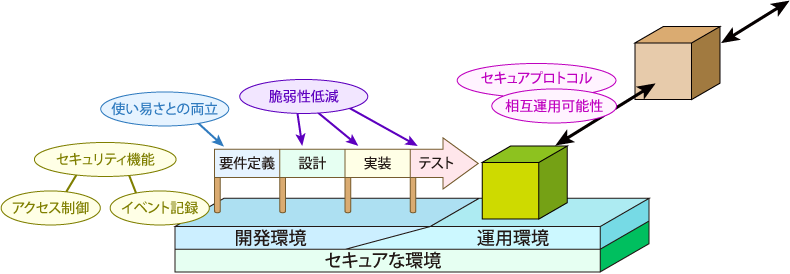
\includegraphics[width=0.8\linewidth]{FigsAppendix/security-eng-2.png}
\end{center}
\end{frame}

\begin{frame}
一方で、標準規格は:
\begin{block}{標準規格となるアルゴリズム・プロトコル}
国家や団体の標準文書に載せるために、\alert{安全性・相互接続性・効率性を分析し、安全性や将来性などがある程度確保}されたもの、と言える。
\end{block}

\begin{center}
 $\Downarrow$
\end{center}

すなわち、\underline{標準規格を要件に応じて適切に選択}し、設計・実装を行うことで脆弱性低減、使いやすさとの両立や相互運用可能性の担保が容易になると言える。

\vspace{1ex}

つまり、最新の標準規格とその推奨される利用方法\footnote[frame]{\scriptsize なぜそのように利用するのか・載っているのか、も正しく知っておく必要がある。悪い例は、脆弱性はあるが互換性のために残っているRFC8017のRSAES-PKCS1-v1\_5。}を把握しておくことで、\alert{効率的なセキュリティエンジニアリングが行える}。
\end{frame}

\begin{frame}
 次ページからは、実際のセキュリティ関連標準について紹介する。
\end{frame}


\begin{frame}
\frametitle{PKCS (Public Key Cryptography Standards)}
\begin{block}{PKCSとは?}
RSA Security社\footnote[frame]{\scriptsize RSA暗号を作ったRivest-Shamir-Adlemanの会社。}の研究部門RSA Labsが策定・公開している、公開鍵暗号を中心とする一連のセキュリティ技術標準のこと。比較的古い、\underline{枯れた標準}になる。
\end{block}
\begin{itemize}
 \item \#1,...\#15の15本が存在\footnote[frame]{\scriptsize 破棄・廃盤も含む。}。
 \item 暗号化・署名生成の手続き・アルゴリズム、データフォーマットの規定など、いわゆる「ローレベル」の技術標準が中心。
 \item RSA暗号標準を定める\#1を代表に、重要なものはメンテされ続けている。が、他の新標準規格で代替されるものなどは破棄・管理移譲されている。
\end{itemize}
\end{frame}

\begin{frame}
PKCSは、その名目上「私企業」が策定した技術標準。

しかし、採用された技術は、十分にセキュリティ評価されていると見做されるものが多く、また他の技術標準に採用・移植・継承されている。
特に多くはIETF RFCの管理下へ継承されているようだ。
\end{frame}

\begin{frame}
PKCS文書一覧(1/2)
\begin{table}
\scriptsize
\begin{tabular}{|l|l|p{21ex}|p{40ex}|}
\hline
 & Ver. & 名称 & 内容 \\
\hline\hline
PKCS \#1 & v2.2 & RSA Cryptography Specifications\footnote[frame]{\scriptsize \url{https://tools.ietf.org/html/rfc8017}} & RSA鍵ペアの構造、暗号化手法、署名手法を策定。\\
\hline
PKCS \#3 & v1.4 & Diffie–Hellman Key Agreement Standard & Diffie-Hellman鍵交換の仕様を策定。RFCではInternet Key Exchange (IKE)へ継承(?)。\\
\hline
PKCS \#5 & v2.1 & Password-Based Cryptography Specification\footnote[frame]{\scriptsize \url{https://tools.ietf.org/html/rfc8018}} & パスワードからの鍵導出手法、暗号化手法 (PBKDF1/2, PBES1/2) の策定。\\
\hline
PKCS \#6 & 廃止 & Extended-Certificate Syntax Standard & X.509v1証明書の拡張。X.509v3へ統合されて廃止。\\
\hline
PKCS \#7 & 廃止(?) & Cryptographic Message Syntax Standard\footnote[frame]{\scriptsize \url{https://tools.ietf.org/html/rfc2315}} & 暗号メッセージ構文を策定。S/MIMEに利用。より新しい仕様 (RFC5652) により廃止(?)。\\
\hline
PKCS \#8 & 廃止(?) & Private-Key Information Syntax Specification\footnote[frame]{\scriptsize \url{https://tools.ietf.org/html/rfc5208}} & 秘密鍵フォーマットを策定。より新しい仕様 (RFC5968) によりv1.2で廃止(?)。\\
\hline
PKCS \#9 & v2.0 & Selected Object Classes and Attribute Types\footnote[frame]{\scriptsize \url{https://tools.ietf.org/html/rfc2985}} & 各種フォーマットにおける「属性」タイプを策定。\\
\hline
\end{tabular}
\end{table}
\end{frame}

\begin{frame}
PKCS文書一覧(2/2)
\begin{table}
\scriptsize
\begin{tabular}{|l|l|p{21ex}|p{40ex}|}
\hline
 & Ver. & 名称 & 内容 \\
\hline\hline
PKCS \#10 & v1.7 & Certification Request Syntax Specification\footnote[frame]{\scriptsize \url{https://tools.ietf.org/html/rfc2986} + \url{https://tools.ietf.org/html/rfc5967}} & 証明書リクエスト構文を策定。元はPKCSのみで策定されていたが、利用されるメディアタイプをRFC5967で拡張。\\
\hline
PKCS \#11 & v2.40 & Cryptographic Token Interface & Cryptokiとしても知られる、暗号トークン(H/Wセキュリティモジュール)インターフェースの仕様を策定。OASIS PKCS 11 Technical Committeeへ継承。\\
\hline
PKCS \#12 & v1.1 & Personal Information Exchange Syntax Standard\footnote[frame]{\scriptsize \url{https://tools.ietf.org/html/rfc7292}} & パスワード暗号化された秘密鍵、公開鍵証明書の構文を策定。IETF IESG管理下へ継承。\\
\hline
PKCS \#15 & v1.1 & Cryptographic Token Information Format Standard & 暗号トークン向け、ユーザ特定標準仕様の策定。ICカード部分はISO/IEC 7816-15へ移譲。\\
\hline
\end{tabular}
\end{table}
策定中のまま立ち消えたものなどは削除。

IETF RFCなどへRepublication、あるいは継承されて新しい標準になっている。
\end{frame}

\begin{frame}
\frametitle{NIST FIPS および SP800\footnote[frame]{参考: https://www.ipa.go.jp/security/publications/nist/}}
\begin{block}{NIST FIPS/SP800とは?}
米国国立標準技術研究所 (NIST; National Institute of Standards and Technology) の発行する文書のこと。
\begin{itemize}
 \item \alert{FIPS; Federal Information Processing Standards}: 米国商務長官の承認の下、NISTが公布した情報セキュリティ関連の米国の標準規格文書。詳細な基準や要求事項、ガイドラインが記載されている。
 \item SP800; Special Publication: 米国政府がセキュリティ対策を実施する際に参考とすることを前提とした、コンピュータセキュリティ関係のレポート。
\end{itemize}
\end{block}
\end{frame}

\begin{frame}
すなわちNIST FIPSは、米国ローカルの標準規格と言える。

\begin{itemize}
\item 多くは、他の国別標準規格同様にANSI/ISO/IEEE等で広く使われていた既存規格を引き継ぐ。
\item 一部はNIST FIPS独自に公募・評価・策定した独自規格。代表的なものは、公募されてきた`Rijndael'という新暗号アルゴリズムを採用したFIPS 197; Advanced Encryption Standard (AES)。
\end{itemize}
\end{frame}

\begin{frame}
\frametitle{IETF RFC (Request for Comments)}
\end{frame}

\begin{frame}
\frametitle{その他; 各国の推奨技術リストとしての標準規格}
\small
\begin{itemize}
 \item CRYPTOREC\footnote[frame]{\scriptsize Cryptography Research and Evaluation Committee} \\
電子政府推奨暗号リストを作り、その実装や運用方法も含めて安全性を調査・評価・監視・検討するプロジェクト (2000年〜)
 \item NESSIE\footnote[frame]{\scriptsize New European Schemes for Signature, Integrity, and Encryption}\\
EUの制定した暗号標準リストを策定するプロジェクト (2000年〜)
\end{itemize}
基本的には、「評価検討した結果、\underline{既存}の暗号アルゴリズム・プロトコルのどれそれを標準として採用する」という\alert{「推奨技術リスト」の策定プロジェクト}だと思って差し支えない。
\end{frame}

\begin{frame}
\small
 
\begin{block}{\small 「各国独自」という意味}
推奨技術リストへ採用されたアルゴリズム・プロトコルは、「その国において正しく評価された比較的安全なもの」というお墨付きを得る。


\underline{セキュリティ技術は国防上重要な意味を持つ}ため、このお墨付きは、その技術を自国で利用して良いものかどうかを判定するもの、と言える。
\end{block}

仕様の詳細はIETF (RFC), ISO, NIST公募など国際的に比較的オープンな場でまず評価・採用・策定される\footnote[frame]{\scriptsize 例外は存在する。元々PKCSはRSA Labs.の独自標準を公開したものだったが、IETFの公開の場でInternet Draftの形で標準化されてきている。}。

\vspace{1ex}

その後、各国が独自に調査検討して推奨技術リストとして採用する、というケースが多い。

\end{frame}


\begin{frame}
\frametitle{公開鍵・秘密鍵のフォーマット・エンコーディング}
\begin{itemize}
 \item PEM
 \item DER
 \item JWK
 \item {[ECC鍵のみ]}  RAW (Octet form)
\end{itemize}
JSの基本はJWK。OpenSSLやSSHなどで馴染みがあるのはPEM。
\end{frame}

\begin{frame}
\frametitle{ECDH, ECDSAの鍵選択(曲線の選択)}
どの曲線を使えばいいのか?
\begin{itemize}
 \item P-256,
 \item P-256K, (Bitcoinで利用)
 \item P-384,
 \item P-521
\end{itemize}
あたりが無難なところ。
\end{frame}




% %%%%%%%%%%%%%%%%%%%%%%%%%%%%%%%%%%%%%%%%%%%%%%%%%%%%%%%%%%%%%%%%%%%%%%%%%%%%%%%%%%%%%%%%%%%%%%%%%%%
% \backupbegin

% \section{Backup}
% \begin{frame}
%  以下バックアップ
% \end{frame}


% \begin{frame}
 
% \end{frame}

% \begin{frame}
% \frametitle{Appendix}
% This page is not counted.
% \end{frame}
% \backupend
\end{document}
%%%%%%%%%%%%%%%%%%%%%%%%%%%%%%%%%%%%%%%%%%%%%%%%%%%%%%%%%%%%%%%%%%%%%%%%%%%%%%%%%%%%%%%%%%%%%%%%%%%
%%%%%%%%%%%%%%%%%%%%%%%%%%%%%%%%%%%%%%%%%%%%%%%%%%%%%%%%%%%%%%%%%%%%%%%%%%%%%%%%%%%%%%%%%%%%%%%%%%%
%%%%%%%%%%%%%%%%%%%%%%%%%%%%%%%%%%%%%%%%%%%%%%%%%%%%%%%%%%%%%%%%%%%%%%%%%%%%%%%%%%%%%%%%%%%%%%%%%%%
%%%%%%%%%%%%%%%%%%%%%%%%%%%%%%%%%%%%%%%%%%%%%%%%%%%%%%%%%%%%%%%%%%%%%%%%%%%%%%%%%%%%%%%%%%%%%%%%%%%
%%%%%%%%%%%%%%%%%%%%%%%%%%%%%%%%%%%%%%%%%%%%%%%%%%%%%%%%%%%%%%%%%%%%%%%%%%%%%%%%%%%%%%%%%%%%%%%%%%%
%%%%%%%%%%%%%%%%%%%%%%%%%%%%%%%%%%%%%%%%%%%%%%%%%%%%%%%%%%%%%%%%%%%%%%%%%%%%%%%%%%%%%%%%%%%%%%%%%%%
